\documentclass[border=10pt,tikz]{standalone}
% Shared palette and styles for the Quota diagrams.
\usepackage{tikz}
\usepackage[T1]{fontenc}
\usepackage{helvet}
\renewcommand{\familydefault}{\sfdefault}
\usetikzlibrary{positioning,fit,backgrounds,arrows.meta,calc,shapes.geometric,shapes.symbols,decorations.pathreplacing,patterns}

\definecolor{qink}{HTML}{14110E}
\definecolor{qorange}{HTML}{E05A28}
\definecolor{qorangelt}{HTML}{FBE7DC}
\definecolor{qcream}{HTML}{FBF7F1}
\definecolor{qgrey}{HTML}{6B6560}
\definecolor{qline}{HTML}{C9C2B8}
\definecolor{qblue}{HTML}{1F5F8B}
\definecolor{qbluelt}{HTML}{DCE8F1}
\definecolor{qgreen}{HTML}{2F6B4F}
\definecolor{qgreenlt}{HTML}{DEEBE3}
\definecolor{qpaper}{HTML}{FFFFFF}

\tikzset{
  box/.style   = {rounded corners=2pt, draw=qline, line width=0.5pt, fill=qpaper,
                  align=center, inner sep=4pt, font=\scriptsize, text=qink},
  src/.style   = {box, minimum height=12mm, text width=25mm},
  proc/.style  = {box, minimum height=10mm, text width=30mm},
  gate/.style  = {box, draw=qorange, line width=1pt, fill=qorangelt},
  store/.style = {box, draw=qink, line width=0.8pt, fill=qcream},
  elas/.style  = {box, draw=qblue, line width=0.7pt, fill=qbluelt},
  human/.style = {box, draw=qgreen, line width=0.7pt, fill=qgreenlt},
  band/.style  = {font=\scriptsize\bfseries, text=qgrey, anchor=east, align=right},
  tag/.style   = {font=\tiny, text=qgrey, align=center, inner sep=1pt},
  ttl/.style   = {font=\scriptsize\bfseries, text=qink},
  flow/.style  = {-{Stealth[length=4pt,width=3pt]}, draw=qgrey, line width=0.7pt},
  flowo/.style = {-{Stealth[length=4pt,width=3pt]}, draw=qorange, line width=1pt},
  flowb/.style = {-{Stealth[length=4pt,width=3pt]}, draw=qblue, line width=0.9pt},
  flowg/.style = {-{Stealth[length=4pt,width=3pt]}, draw=qgreen, line width=0.9pt},
  dash/.style  = {draw=qline, line width=0.5pt, dash pattern=on 2pt off 2pt},
  grp/.style   = {rounded corners=3pt, draw=qline, line width=0.5pt, fill=qcream, inner sep=5pt},
}
\newcommand{\bb}[1]{\textbf{#1}}
\newcommand{\gy}[1]{{\color{qgrey}#1}}

\begin{document}
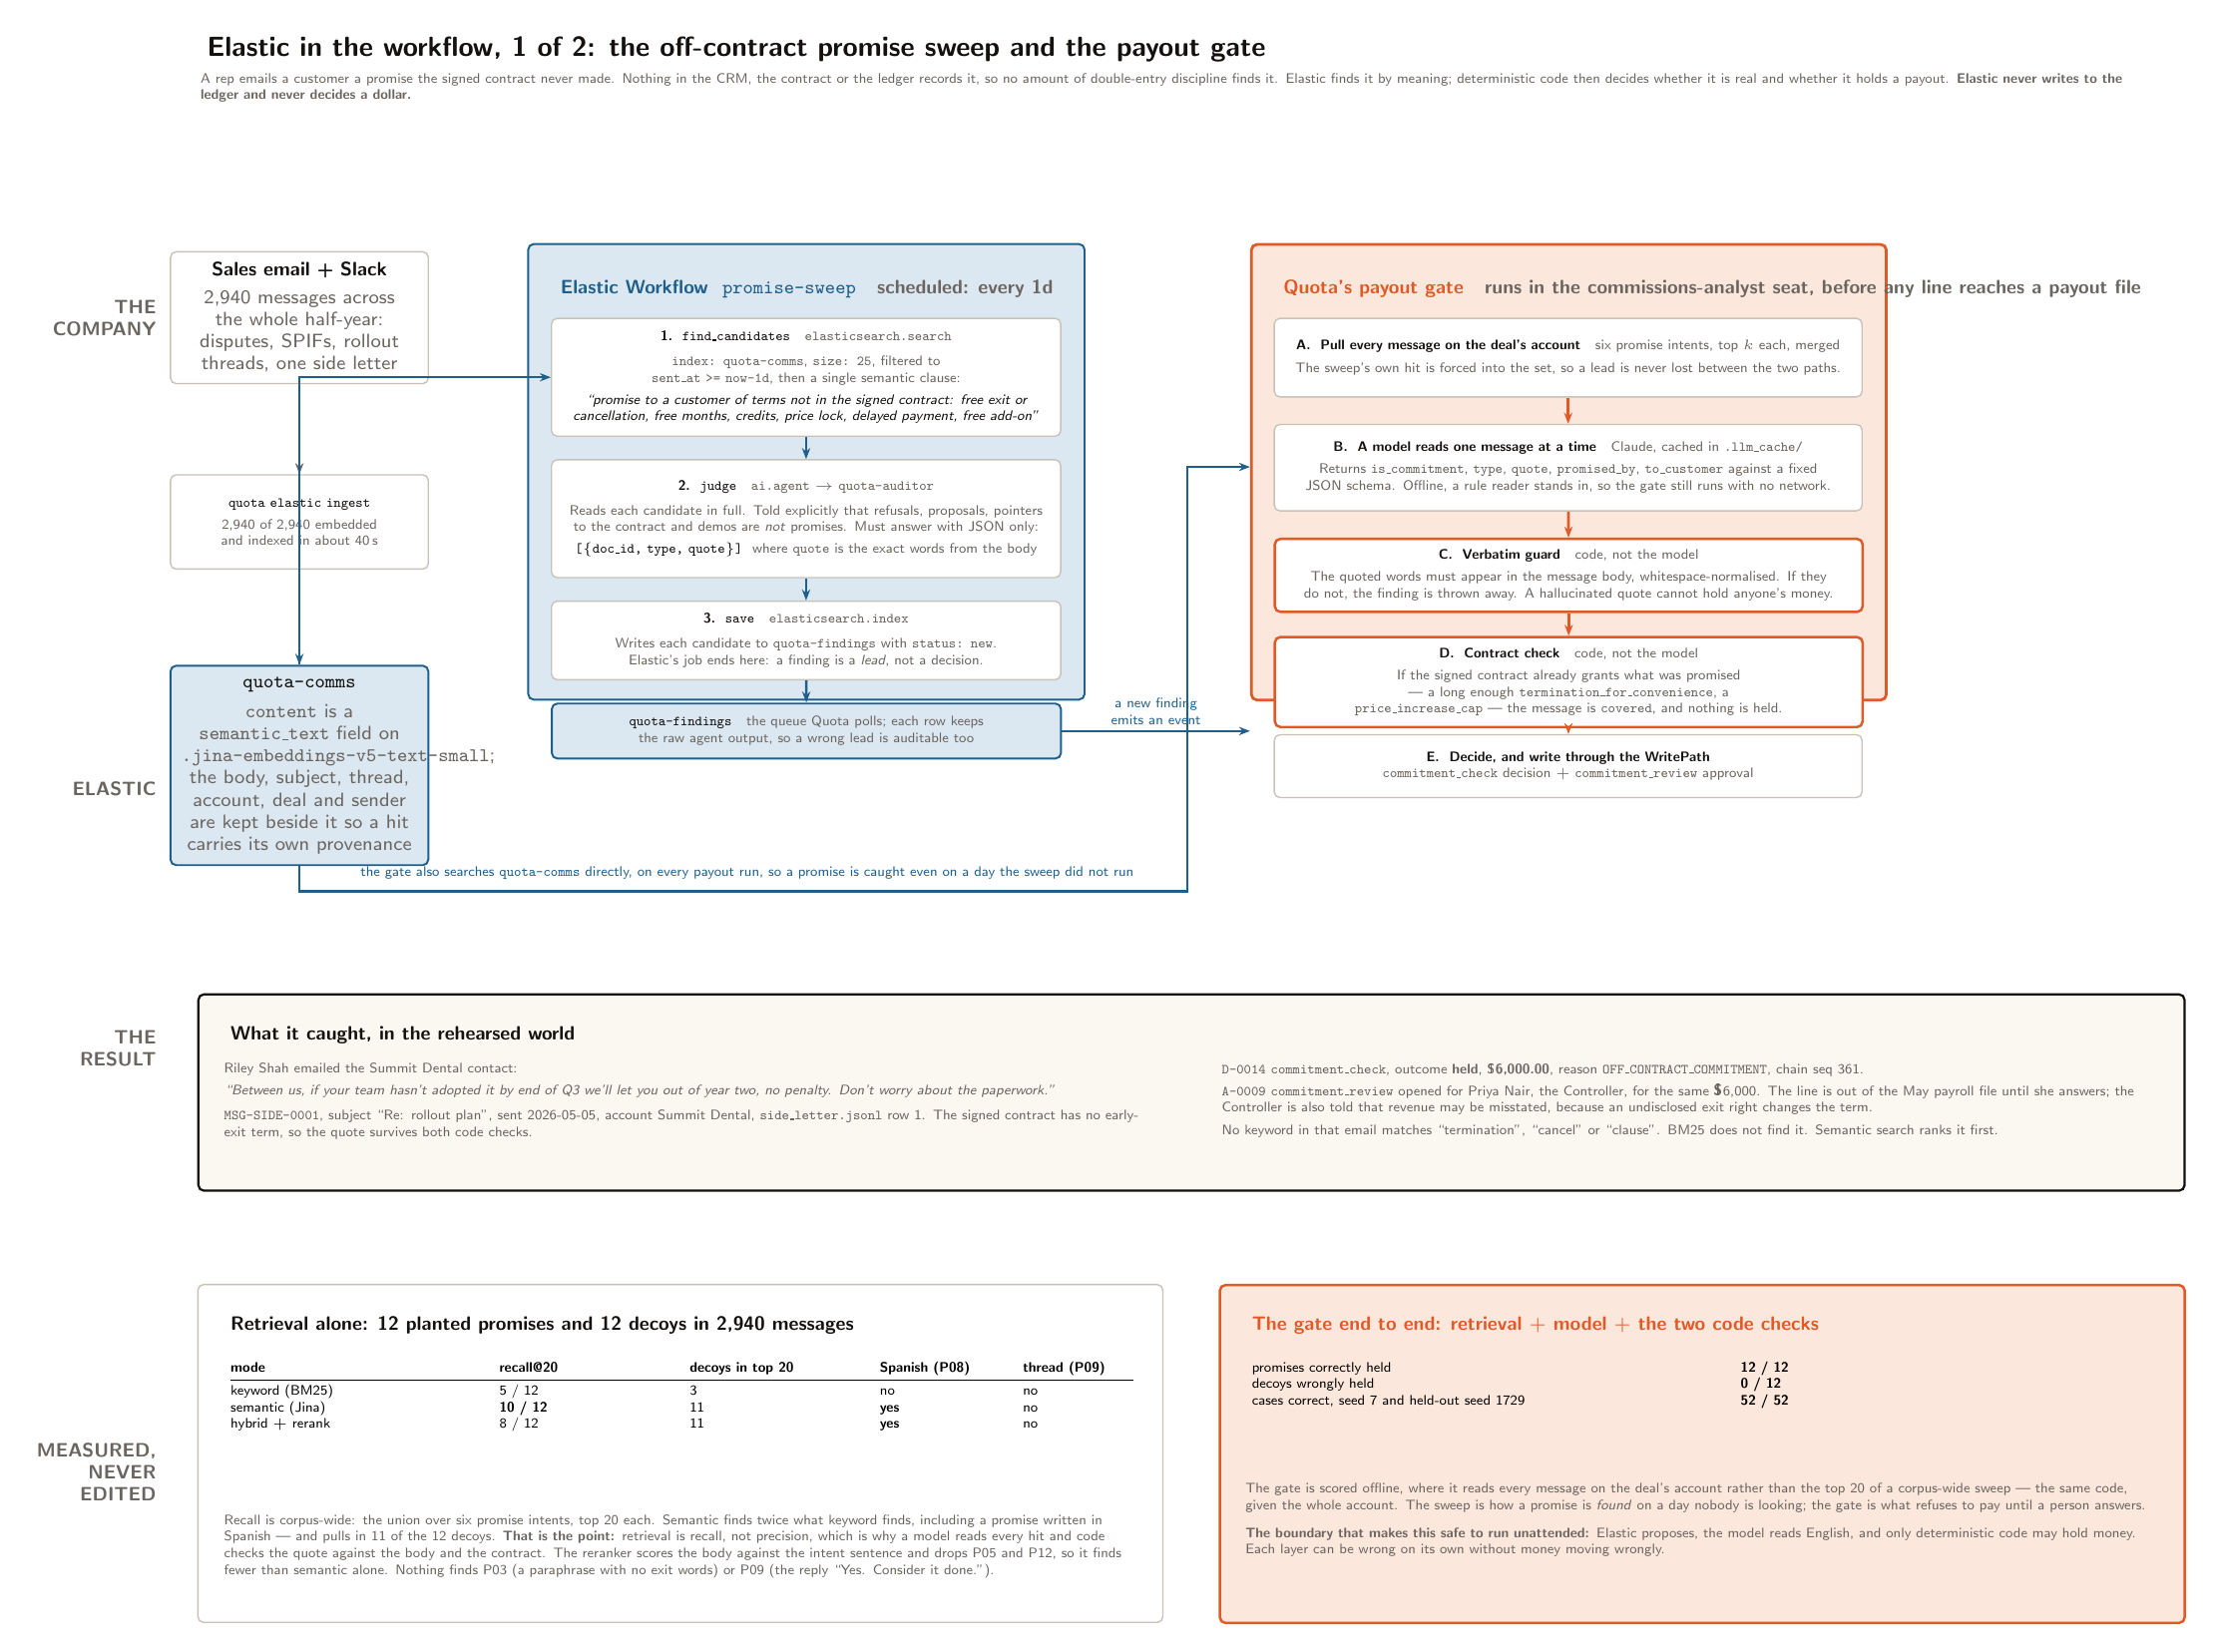
\begin{tikzpicture}[x=1cm,y=1cm]

\node[ttl, anchor=north west, font=\normalsize\bfseries] at (0,0.4) {Elastic in the workflow, 1 of 2: the off-contract promise sweep and the payout gate};
\node[tag, anchor=north west, align=left, text width=250mm] at (0,-0.15)
  {{\color{qgrey}A rep emails a customer a promise the signed contract never made. Nothing in the CRM, the contract or the ledger records it, so no amount of double-entry discipline finds it. Elastic finds it by meaning; deterministic code then decides whether it is real and whether it holds a payout. \textbf{Elastic never writes to the ledger and never decides a dollar.}}};

%====================== 1. CORPUS ======================
\node[band] at (-0.4,-3.3) {THE\\COMPANY};
\node[src, text width=30mm, minimum height=16mm] at (1.3,-3.3) (corpus)
  {\bb{Sales email + Slack}\\[2pt]{\color{qgrey}2{,}940 messages across\\the whole half-year:\\disputes, SPIFs, rollout\\threads, one side letter}};
\node[box, text width=30mm, minimum height=12mm, font=\tiny] at (1.3,-5.9) (ingest)
  {\bb{\texttt{quota elastic ingest}}\\[2pt]{\color{qgrey}2{,}940 of 2{,}940 embedded\\and indexed in about 40\,s}};
\draw[flow] (corpus) -- (ingest);

%====================== 2. INDEX ======================
\node[band] at (-0.4,-9.3) {ELASTIC};
\node[elas, text width=30mm, minimum height=22mm] at (1.3,-9.0) (comms)
  {\bb{\texttt{quota-comms}}\\[3pt]{\color{qgrey}\texttt{content} is a \texttt{semantic\_text} field on \texttt{.jina-embeddings-v5-text-small}; the body, subject, thread, account, deal and sender are kept beside it so a hit carries its own provenance}};
\draw[flowb] (ingest) -- (comms);

%====================== 3. THE WORKFLOW ======================
\node[elas, text width=68mm, minimum height=58mm, anchor=north west] at (4.2,-2.35) (wf) {};
\node[ttl, anchor=north west, text=qblue] at (4.5,-2.7) {Elastic Workflow \ \texttt{promise-sweep} \ \ {\color{qgrey}\scriptsize scheduled: every 1d}};

\node[box, text width=62mm, minimum height=15mm, font=\tiny, anchor=north west] at (4.5,-3.3) (w1)
  {\bb{1.\ \ \texttt{find\_candidates}} \ \ {\color{qgrey}\texttt{elasticsearch.search}}\\[3pt]
   {\color{qgrey}\texttt{index: quota-comms}, \texttt{size: 25}, filtered to \texttt{sent\_at >= now-1d}, then a single semantic clause:}\\[2pt]
   \textit{``promise to a customer of terms not in the signed contract: free exit or cancellation, free months, credits, price lock, delayed payment, free add-on''}};

\node[box, text width=62mm, minimum height=15mm, font=\tiny, anchor=north west] at (4.5,-5.1) (w2)
  {\bb{2.\ \ \texttt{judge}} \ \ {\color{qgrey}\texttt{ai.agent} $\rightarrow$ \texttt{quota-auditor}}\\[3pt]
   {\color{qgrey}Reads each candidate in full. Told explicitly that refusals, proposals, pointers to the contract and demos are \emph{not} promises. Must answer with JSON only:}\\[2pt]
   \texttt{[\{doc\_id, type, quote\}]} \ {\color{qgrey}where \texttt{quote} is the exact words from the body}};

\node[box, text width=62mm, minimum height=10mm, font=\tiny, anchor=north west] at (4.5,-6.9) (w3)
  {\bb{3.\ \ \texttt{save}} \ \ {\color{qgrey}\texttt{elasticsearch.index}}\\[3pt]
   {\color{qgrey}Writes each candidate to \texttt{quota-findings} with \texttt{status: new}. Elastic's job ends here: a finding is a \emph{lead}, not a decision.}};

\node[elas, text width=62mm, minimum height=7mm, font=\tiny, anchor=north west] at (4.5,-8.2) (findings)
  {\bb{\texttt{quota-findings}} \ \ {\color{qgrey}the queue Quota polls; each row keeps the raw agent output, so a wrong lead is auditable too}};

\draw[flowb] (w1) -- (w2);
\draw[flowb] (w2) -- (w3);
\draw[flowb] (w3) -- (findings);
\draw[flowb] (comms.north) |- ($(w1.west)+(-0.35,0)$) -- (w1.west);


%====================== 4. THE GATE ======================
\node[band] at (13.1,-1.0) {};
\node[gate, text width=78mm, minimum height=58mm, anchor=north west] at (13.4,-2.35) (gatebox) {};
\node[ttl, anchor=north west, text=qorange] at (13.7,-2.7) {Quota's payout gate \ \ {\color{qgrey}\scriptsize runs in the commissions-analyst seat, before any line reaches a payout file}};

\node[box, text width=72mm, minimum height=10mm, font=\tiny, anchor=north west] at (13.7,-3.3) (g1)
  {\bb{A.\ \ Pull every message on the deal's account} \ \ {\color{qgrey}six promise intents, top $k$ each, merged}\\[2pt]
   {\color{qgrey}The sweep's own hit is forced into the set, so a lead is never lost between the two paths.}};

\node[box, text width=72mm, minimum height=11mm, font=\tiny, anchor=north west] at (13.7,-4.65) (g2)
  {\bb{B.\ \ A model reads one message at a time} \ \ {\color{qgrey}Claude, cached in \texttt{.llm\_cache/}}\\[2pt]
   {\color{qgrey}Returns \texttt{is\_commitment}, \texttt{type}, \texttt{quote}, \texttt{promised\_by}, \texttt{to\_customer} against a fixed JSON schema. Offline, a rule reader stands in, so the gate still runs with no network.}};

\node[box, draw=qorange, line width=0.9pt, text width=72mm, minimum height=9mm, font=\tiny, anchor=north west] at (13.7,-6.1) (g3)
  {\bb{C.\ \ Verbatim guard} \ \ {\color{qgrey}code, not the model}\\[2pt]
   {\color{qgrey}The quoted words must appear in the message body, whitespace-normalised. If they do not, the finding is thrown away. A hallucinated quote cannot hold anyone's money.}};

\node[box, draw=qorange, line width=0.9pt, text width=72mm, minimum height=9mm, font=\tiny, anchor=north west] at (13.7,-7.35) (g4)
  {\bb{D.\ \ Contract check} \ \ {\color{qgrey}code, not the model}\\[2pt]
   {\color{qgrey}If the signed contract already grants what was promised \textemdash{} a long enough \texttt{termination\_for\_convenience}, a \texttt{price\_increase\_cap} \textemdash{} the message is \texttt{covered}, and nothing is held.}};

\node[box, text width=72mm, minimum height=8mm, font=\tiny, anchor=north west] at (13.7,-8.6) (g5)
  {\bb{E.\ \ Decide, and write through the WritePath} \ \ {\color{qgrey}\texttt{commitment\_check} decision $+$ \texttt{commitment\_review} approval}};

\draw[flowo] (g1) -- (g2);
\draw[flowo] (g2) -- (g3);
\draw[flowo] (g3) -- (g4);
\draw[flowo] (g4) -- (g5);
\draw[flowb] (findings.east) -- node[tag,midway,above=1pt,font=\tiny,text=qblue,align=center]{a new finding\\emits an event} (gatebox.west|-findings);
\draw[flowb] (comms.south) -- (1.3,-10.6) -- (12.6,-10.6) -- (12.6,-5.2) -- (gatebox.west|-{(0,-5.2)});
\node[tag, anchor=south, font=\tiny, text=qblue, align=center] at (7.0,-10.5) {the gate also searches \texttt{quota-comms} directly, on every payout run, so a promise is caught even on a day the sweep did not run};

%====================== 5. OUTCOME ======================
\node[band] at (-0.4,-12.6) {THE\\RESULT};
\node[box, draw=qink, line width=0.8pt, fill=qcream, text width=250mm, minimum height=25mm, anchor=north west] at (0,-11.9) (out) {};
\node[ttl, anchor=north west] at (0.3,-12.2) {What it caught, in the rehearsed world};
\node[tag, anchor=north west, align=left, text width=118mm] at (0.3,-12.75)
  {{\color{qgrey}Riley Shah emailed the Summit Dental contact:}\\[2pt]
   \textit{``Between us, if your team hasn't adopted it by end of Q3 we'll let you out of year two, no penalty. Don't worry about the paperwork.''}\\[3pt]
   {\color{qgrey}\texttt{MSG-SIDE-0001}, subject ``Re: rollout plan'', sent 2026-05-05, account Summit Dental, \texttt{side\_letter.jsonl} row 1. The signed contract has no early-exit term, so the quote survives both code checks.}};
\node[tag, anchor=north west, align=left, text width=118mm] at (13.0,-12.75)
  {\bb{\texttt{D-0014}} {\color{qgrey}\texttt{commitment\_check}, outcome} \bb{held}, \bb{\$6{,}000.00}, {\color{qgrey}reason} \texttt{OFF\_CONTRACT\_COMMITMENT}{\color{qgrey}, chain seq 361.}\\[2pt]
   \bb{\texttt{A-0009}} {\color{qgrey}\texttt{commitment\_review} opened for Priya Nair, the Controller, for the same \$6{,}000. The line is out of the May payroll file until she answers; the Controller is also told that revenue may be misstated, because an undisclosed exit right changes the term.}\\[2pt]
   {\color{qgrey}No keyword in that email matches ``termination'', ``cancel'' or ``clause''. BM25 does not find it. Semantic search ranks it first.}};

%====================== 6. MEASURED ======================
\node[band] at (-0.4,-18.0) {MEASURED,\\NEVER\\EDITED};
\node[box, text width=120mm, minimum height=43mm, anchor=north west] at (0,-15.6) (ev1) {};
\node[ttl, anchor=north west] at (0.3,-15.9) {Retrieval alone: 12 planted promises and 12 decoys in 2{,}940 messages};
\node[anchor=north west, font=\tiny] at (0.3,-16.45) {%
  \begin{tabular}{@{}p{30mm}p{20mm}p{20mm}p{14mm}p{14mm}@{}}
  \textbf{mode} & \textbf{recall@20} & \textbf{decoys in top 20} & \textbf{Spanish (P08)} & \textbf{thread (P09)}\\[1pt]
  \hline\\[-5pt]
  keyword (BM25) & 5 / 12 & 3 & no & no\\
  semantic (Jina) & \textbf{10 / 12} & 11 & \textbf{yes} & no\\
  hybrid $+$ rerank & 8 / 12 & 11 & \textbf{yes} & no\\
  \end{tabular}};
\node[tag, anchor=north west, align=left, text width=115mm] at (0.3,-18.5)
  {{\color{qgrey}Recall is corpus-wide: the union over six promise intents, top 20 each. Semantic finds twice what keyword finds, including a promise written in Spanish \textemdash{} and pulls in 11 of the 12 decoys. \textbf{That is the point:} retrieval is recall, not precision, which is why a model reads every hit and code checks the quote against the body and the contract. The reranker scores the body against the intent sentence and drops P05 and P12, so it finds fewer than semantic alone. Nothing finds P03 (a paraphrase with no exit words) or P09 (the reply ``Yes. Consider it done.'').}};

\node[box, draw=qorange, line width=0.9pt, fill=qorangelt, text width=120mm, minimum height=43mm, anchor=north west] at (13.0,-15.6) (ev2) {};
\node[ttl, anchor=north west, text=qorange] at (13.3,-15.9) {The gate end to end: retrieval $+$ model $+$ the two code checks};
\node[anchor=north west, font=\tiny] at (13.3,-16.45) {%
  \begin{tabular}{@{}p{58mm}p{25mm}@{}}
  promises correctly held & \textbf{12 / 12}\\
  decoys wrongly held & \textbf{0 / 12}\\
  cases correct, seed 7 and held-out seed 1729 & \textbf{52 / 52}\\
  \end{tabular}};
\node[tag, anchor=north west, align=left, text width=115mm] at (13.3,-18.1)
  {{\color{qgrey}The gate is scored offline, where it reads every message on the deal's account rather than the top 20 of a corpus-wide sweep \textemdash{} the same code, given the whole account. The sweep is how a promise is \emph{found} on a day nobody is looking; the gate is what refuses to pay until a person answers.}\\[4pt]
   \bb{The boundary that makes this safe to run unattended:} {\color{qgrey}Elastic proposes, the model reads English, and only deterministic code may hold money. Each layer can be wrong on its own without money moving wrongly.}};

\end{tikzpicture}
\end{document}
